\documentclass[a4paper,8pt,twocolumn]{extarticle}
\usepackage[utf8]{inputenc}
\usepackage{graphicx}
\usepackage[center]{caption}
\usepackage[english]{babel}
\usepackage[top=2cm, bottom=2cm, left=2cm, right=2cm]{geometry}

%---------------------------------------------
% Font packages
%---------------------------------------------
\usepackage{lmodern}
% \usepackage{concmath}
% \usepackage{cmbright}
% \usepackage{kpfonts}
% \usepackage[adobe-utopia]{mathdesign}
% \usepackage{fouriernc}
\usepackage[T1]{fontenc}

%---------------------------------------------
% Math environment packages & command
%---------------------------------------------
\usepackage{amsmath}
\usepackage{amssymb}
\usepackage{array}
% \usepackage{mathrsfs}
\usepackage{array}
% \def\sgn{\mathop{\rm sgn}\nolimits} 
% \usepackage{bbm}


%---------------------------------------------
% item option
%---------------------------------------------
\renewcommand{\labelitemi}{-}


%---------------------------------------------
%HEADER & FOOTER
%---------------------------------------------
\usepackage{fancyhdr}
\pagestyle{fancy}

\renewcommand{\headrulewidth}{.15pt}
\fancyhead[C]{{\textsc{The Guarding Problem}}} 
\fancyhead[L]{Page \thepage \ of \pageref{LastPage}}
\fancyhead[R]{DD2438}

\renewcommand{\footrulewidth}{.15pt}
\fancyfoot[C]{\thepage} 
% \fancyfoot[L]{truc}
% \fancyfoot[R]{bidule}

\usepackage{lastpage}

%---------------------------------------------
% two column option
%---------------------------------------------
\setlength{\columnsep}{0.7cm}

%---------------------------------------------
% Table of content
%---------------------------------------------
\usepackage[colorlinks,linkcolor=black, citecolor=black]{hyperref}

%---------------------------------------------
% Opening
%---------------------------------------------
\title{Artificial Intelligence \& Multi-Agent System :\\ \textsc{The Guarding Problem}}
\author{Björn \textsc{Holm}, Kilian \textsc{Demeulemeester} \\ \texttt{\{bjh,kiliande\}@kth.se}}

%---------------------------------------------
% Numerotation Handling
%---------------------------------------------
 %\setcounter{section}{3}
 \usepackage[explicit]{titlesec}
  %\titleformat{<command>}[<shape>]{<format>}{<label>}{<sep>}{<before>}[<after>]
	\titleformat{\section}[block]{\normalsize\bfseries\filcenter}{\Roman{section}.}{1em}{#1}
	\titleformat{\subsection}[block]{\normalsize\bfseries}{\emph{\Alph{subsection}.}}{1em}{\emph{#1}}
 %\titleformat{\section}[hang]{\normalfont\Large\bfseries}%
     %{}{8pt}%
     %{\arabic{section}. #1}


%---------------------------------------------
% Dummy text
%---------------------------------------------
\usepackage{lipsum}

%---------------------------------------------
% Bibliography package
%---------------------------------------------
\usepackage{url}

%---------------------------------------------
% Algorithm form
%---------------------------------------------
\newtheorem{algorithm}{Algorithm}[section]
\newtheorem{criteria}{Criteria}[section]
\newtheorem{problem}{Problem}
\newtheorem{subproblem}{Problem}[section]
\newtheorem{definition}{Definition}[section]
\newcommand{\qed}{\hfill $\blacksquare$}

\begin{document}

% % Indentation size
% \setlength\parindent{0em}
% 
% \setlength{\itemsep}{0pt}

\maketitle

% \tableofcontents


\begin{bfseries}
\emph{Abstract} -- 
The purpose of this project was to create an environment -- using \texttt{Unity} -- where vehicules execute cooperativly search and pursuit of intruders. The problem involves optimising different algorithms such as discretizing an environment, computing a minimal path for a fleet of vehicule that are to survey a given area, optimizing the search of a mobile intruder, pursuiting and capturing an intruder.

In this paper we focus on three different problems. The first is how to find the position of static guards such that a given set of building is completly guard. The second problem is how to clean a area with moving guard -- \emph{i.e.} every part of the area has been seen. The third problem is how to search and capture a moving intruder that is trying to escape.
\end{bfseries}


\vspace{0.5cm}
\hrule

\section{The three problems}
Our work was divided into three main problems, even if we tried to keep a high level of generality in order to use as much as possible the different algorithm in the three of them.

\begin{problem}[Static Guarding]
Given an environment, find a set of points $P_{1\leq i \leq n}$ such that every free point in the environment is visible from a least one $P_i$, with $n$ as small as possible. This problem is also known as the art gallery problem.
\end{problem}
\begin{problem}[Dynamic Guarding]
Given an environment, find paths for $n$ robot ($n$ is a parameter) in order to clear the whole area, \emph{i.e} each point in the environment has been seen.
\end{problem}
\begin{problem}[Search \& Capture]
Given an environment, find paths for $n$ robot ($n$ as small as possible) in order to find a moving intruder. Once it is located, pursue and capture it.
\end{problem}

\section{Environment representation}
The environment used is build with Unity as a set of obstacles with all of edges either perpendiculars or parallels.

In order to enhance the performance, we discretize our environment using a grid. Each cell is either \emph{occupied} if one of its corners lies into an obstacle or \emph{free}.

The environment is then covered by a set of convex $C_{1\leq i \leq n}$ with each $C_i$ satisfying the following criteria.

\begin{criteria}[of Visibility]
 \emph{For all point $P$ in the area, if each corner of $C_i$ is visible, then the whole area is visible}. In practice, it means that checking if a convex can be seen from a given point can be done in only $4$ raycasting.
\label{visibilityCriteria}
\end{criteria}

The three problems we investigate involve finding interesting point on the map. We uses the following denomination:
\begin{description}
	\item[Waypoints:] Points at a given distance of each obstacle corners (see Figure \ref{convexCover});
	\item[Points of surveillance:] Points from which all the area is surveyed.
\end{description}

\subsection{Convex set cover}

In order to solve our three problems, we needed a convex cover set of our area. The algorithm used to create the convex set is based on the work from \cite{CoopMinTime}. Figure \ref{convexCover} shows the convex cover generated by the algorithm \ref{algoConvexCover}.

\begin{algorithm}
This algorithm describe how to create a maximal convex cover of our environment. Since the obstacles are all orthogonal, the maximal convex sets $C_i$ are rectangle aligned with the polygon.
\begin{enumerate}
\item Based on the grid, make a discretization of the environment $G(A)$.
\item Find a yet uncovered cell, p.
\item Start growing a rectange $C_i$ from $p$ until its length and/or width reach $R$\footnote{R is the maximum convex size in width and/or length. This parameter is used to guarantee the visibily criteria \ref{visibilityCriteria}}.
\item While uncovered cells exists, goto 2.
\end{enumerate}
\label{algoConvexCover}
\end{algorithm}

\begin{figure}[h!t]
	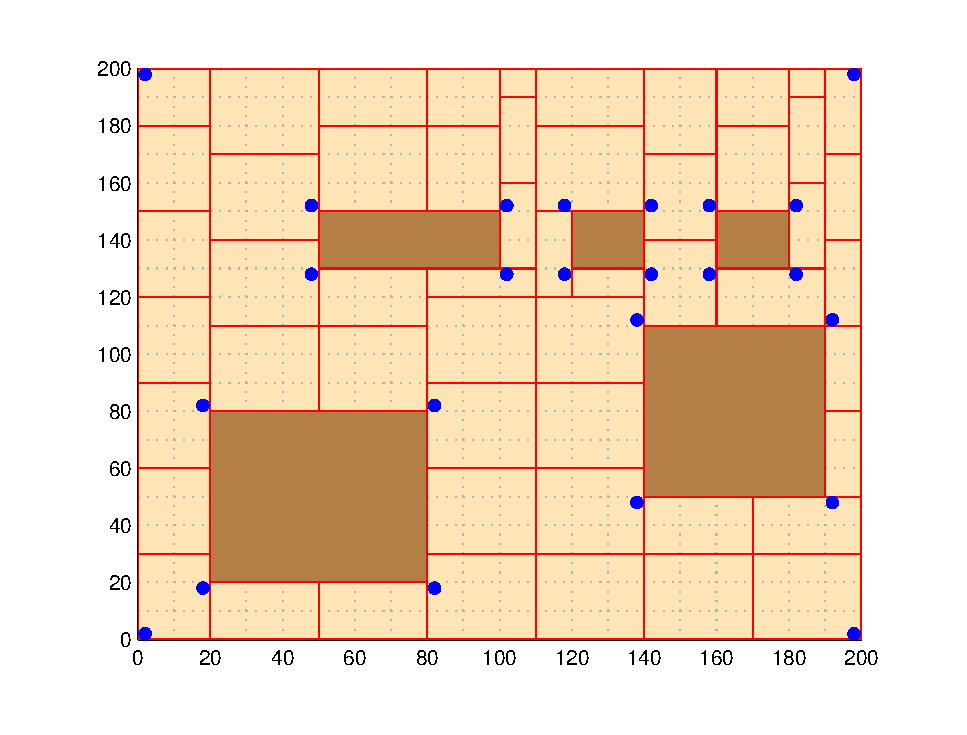
\includegraphics[width=\linewidth]{fig/convexCover.eps}
	\caption{Waypoints of the environment \& Convex set cover}
	\label{convexCover}
\end{figure}


\subsection{Graph representation \& search}

\textsc{About graph generation from the environment using waypoints and the $A^{\ast}$ algorithm!}


\section{Static Guarding}
This problem is solved using the greedy algorithm \ref{algStaticGuard}, which generate a set of point $ S = P_{1\leq i \leq n}$ from which the environment is completely visible. Figure \ref{convexTesselation} shows the set of points produced by the algorithm.

\begin{algorithm}
This algorithm gives a way to find a set of points from which the environment is completely visible.
\begin{enumerate}
	\item Generate a set of potential points (we used the center of every grid cell).
	\item Create a set of unseen areas $U_i = C_i$ (see alg. \ref{algoConvexTesselation}).
	\item Find the point $p$ from which most of the area is visible.
	\item Add this point to the set of point $S$.
	\item Remove areas visible from $p$ from $U$.
	\item While there are unseen areas left, go to 3.
\end{enumerate}
\label{algStaticGuard}
\end{algorithm}

Even if there is no guarantee that algorithm \ref{algStaticGuard} will find the optimal solution, its low complexity ($\mathcal{O}(n)$ -- where $n$ is the size of the set) has been proven to be the best-possible polynomial time approximation algorithm for set cover (see \cite{approxMinProb}).

\begin{figure}[h!t]
	\begin{center}
	\includegraphics[width=\linewidth,natwidth=824,natheight=823]{fig/staticCoverSet.jpg}
	\end{center}
	\caption{Set cover \& Positions for static guarding}
	\label{convexTesselation}
\end{figure}


\section{Dynamic Guarding}
The problem of dynamic guarding we approach by first solving the static guarding problem, giving us a set of points that are sufficient for surveiling the whole environment.
All we have to do now is visit all of these points with at least one guard, this is the Vehicle Routing Problem, VRP.

This may not yield an optimal solution, but a solution none the less.


\section{Search \& Destroy}
We here only have an idea for an algorithm for solving this problem, it is not yet tested.

The algorithm is based an algorithm for solving the same problem in \cite{multiSearchSecure}, and the basic idea is to first place guards to break the problem down into smaller problems until a single guard can completely secure the smaller problem.
Once an area has been secured, it should never be allowed to be directly connected to unsecured areas again, but as long as this is satisfied, all guards may move around.
After securing an area, again try to break down the remaining problem into smaller problems and recurse.

\ \\
Each area has two different boolean properties:
\begin{definition}[Watched]
if at least one guard can see the whole area.
\end{definition}
\begin{definition}[Secured]
if all of it's neighbors are either secured or watched.
\end{definition}
\\
Each guard only has one property:
\begin{definition}[Occupied]
if it is the only guard watching an area that is not secured itself, but connected to both secured and unsecured areas.
\end{itemize}

\begin{algorithm}
This is an algorithm for finding the points for guards to visit in order to secure a given 2D vector environment divided into free-space and obstacles. Intruders are allowed to move arbitrarily fast.

The algorithm is greedy, but corresponding versions of searching for and evaluating different solutions could also be made.
\begin{enumerate}
	\item Tesselate the environment into convex polygons and generate a walkability-graph of the connected polygons. (see Figure \ref{searchDestroy})
	\item Somehow find a point $p$ which divides the graph into smaller graphs. (see Figure \ref{searchDestroy2})
			Preferably, at least one of the smaller graphs should be of a size smaller than the number of currently available unoccupied guards.
	\item Move an unoccupied guard to $p$, if all guards are occupied, add a new guard at $p$.
	\item If all the areas are either secured or watched, we are done, otherwise, goto 2.
\end{enumerate}
\label{algSearchDestroyIdea}
\end{algorithm}

The possible points to visit and how placing a guard at that point transforms the walkability-graph could possibly be pre-generated.

%\begin{figure}[h!t]
%	\includegraphics[width=\linewidth]{fig/2graph.png}
%	\caption{The tesselation (red) and walkability-graph (black) of an environment}
%	\label{searchDestroy}
%\end{figure}

%\begin{figure}[h!t]
%	\includegraphics[width=\linewidth]{fig/2graph2.png}
%	\caption{The new walkability-graph after placing a guard at the cross}
%	\label{searchDestroy2}
%\end{figure}

\section*{Conclusion}
\addcontentsline{toc}{section}{Conclusion}
We have in this report described how we solved the problems of finding a static surveillance (the art gallery problem) and finding patrol paths for moving guards looking for immobile intruders.
We have also given an idea for an algorithm to secure an environment while the intruders are moving around.

None of our solutions are guaranteed to be optimal, but visual inspection suggests them to be quite good.


\nocite{*}
\bibliographystyle{plain}
\bibliography{bibliography}

\end{document}
